\documentclass[../../main.tex]{subfiles}
\graphicspath{{../../image/}{../../figure/}}
\begin{document}

\section{多层网络}\label{section:ch06-多层网络}

考虑具有两层可学习参数的基本神经网络。首先用以下形式构造输入变量 $x_1,\cdots,x_D$ 的 $M$ 个线性组合：
\begin{align}
a_j^{(1)} = \sum_{i=1}^{D} w_{ji}^{(1)} x_i + b_j^{(1)}, \qquad j=1,\cdots,M,
\label{align:ch06-preact1}
\end{align}
其中 $j=1,\cdots,M$，上标 $(1)$ 表示相应参数位于神经网络的第一层。参数 $w_{ji}^{(1)}$ 称为\textbf{权重}（weight），$b_j^{(1)}$ 称为\textbf{偏置}参数（bias），$a_j^{(1)}$ 则称为\textbf{预激活}（pre-activation，参见第~4~章）。然后，每个 $a_j^{(1)}$ 通过一个可微的非线性激活函数 $h(\cdot)$ 被转换为
\begin{align}
z_j^{(1)} = h\!\left(a_j^{(1)}\right),
\label{align:ch06-hidden}
\end{align}
它代表~\eqref{align:ch06-linear-basis}~中基函数的输出。在神经网络语境中，这些基函数 $z_j^{(1)}$ 称为\textbf{隐藏单元}（hidden unit）。

只要导数 $h'(\cdot)$ 可以计算，整个网络函数就是可微的。遵循~\eqref{align:ch06-linear-basis}，这些值可以再次被线性组合为
\begin{align}
a_k^{(2)} = \sum_{j=1}^{M} w_{kj}^{(2)} z_j^{(1)} + b_k^{(2)}, \qquad k=1,\cdots,K,
\label{align:ch06-preact2}
\end{align}
其中 $k=1,\cdots,K$，$K$ 是输出总数。该变换对应神经网络的第二层，$w_{kj}^{(2)}$ 同样是权重参数。最后，$a_k^{(2)}$ 通过适当的输出单元激活函数 $f(\cdot)$ 被转换为网络输出 $y_k$。两层神经网络可以用图~\ref{fig:ch06-mlp}~所示的有向图表示。

\begin{figure}[htbp]
\centering
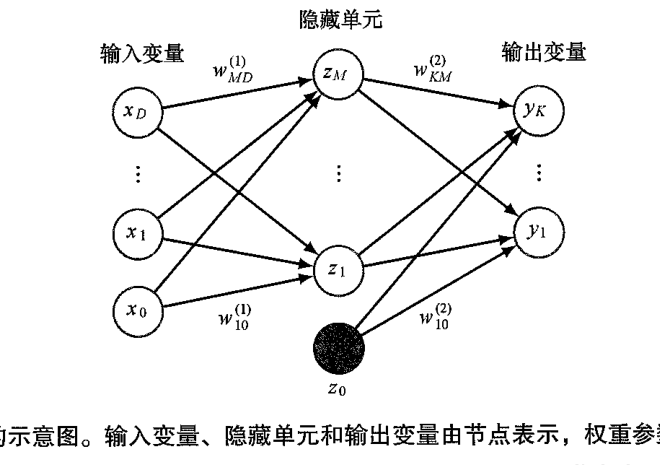
\includegraphics[width=0.55\textwidth]{ch06-fig6-9-mlp.png}
\caption{两层神经网络示意图。输入变量、隐藏单元和输出变量由节点表示，权重参数由节点之间的连接表示。偏置参数由来自额外输入 $x_0=1$ 和隐藏变量 $z_0=1$ 的连接表示；箭头表示前向传播过程中信息流动的方向。}
\label{fig:ch06-mlp}
\end{figure}

\subsection{参数矩阵}\label{section:ch06-参数矩阵}

如~4.1.1~小节所述，通过定义一个额外值恒为 $1$ 的输入变量 $x_0$，可以将~\eqref{align:ch06-preact1}~中的偏置参数吸收到权重参数集合中，使~\eqref{align:ch06-preact1}~变为
\begin{align}
a_j^{(1)} = \sum_{i=0}^{D} w_{ji}^{(1)} x_i.
\label{align:ch06-preact1-biased}
\end{align}

同样也可以把第二层的偏置吸收到第二层权重集合中，于是整个网络函数变为
\begin{align}
z_j^{(1)} = h\!\left(\sum_{i=0}^{D} w_{ji}^{(1)} x_i\right), \qquad
y_k = f\!\left(\sum_{j=0}^{M} w_{kj}^{(2)} z_j^{(1)}\right).
\label{align:ch06-mlp-scalar}
\end{align}

一种方便的表示法是把输入表示为列向量 $\mathbf{x} = (x_1,\cdots,x_D)^{\mathsf T}$，然后将~\eqref{align:ch06-mlp-scalar}~中的权重和偏置参数聚集成矩阵。写 $\mathbf{z}^{(1)} = h(\mathbf{W}^{(1)}\mathbf{x} + \mathbf{b}^{(1)})$，$\mathbf{y} = f(\mathbf{W}^{(2)}\mathbf{z}^{(1)} + \mathbf{b}^{(2)})$，其中 $h(\cdot)$ 和 $f(\cdot)$ 分别逐元素作用于向量。

\subsection{通用近似}\label{section:ch06-通用近似}

图~6.10~展示了两层神经网络近似四种不同函数的能力：$f(x)=x^2$、$f(x)=\sin x$、$f(x)=1/x$ 以及 Heaviside 阶跃函数 $H(x)$。该图还展示了各个隐藏单元如何协作从而近似最终函数；图~6.11~则在一个简单二分类问题中说明了隐藏单元的作用。

20~世纪~80~年代，两层前馈网络的近似性质得到了广泛研究。各种定理表明：对于大多数激活函数而言，这样的网络可以以任意精度近似定义在紧的连续子集上的任何函数~\citep{Funahashi1989,Cybenko1989,HornikStinchcombeWhite1989,Leshno1993}。对于从任意有限维离散空间到另一空间的映射，也有类似结论。因此，神经网络可以视为\textbf{通用近似器}（universal approximator）。

虽然这些定理令人安心，但已有研究只告诉我们\emph{存在}可表示所需函数的网络，并未说明这样的网络能否通过学习算法找到；此外，某些情况下它们可能需要指数级数量的隐藏单元。更重要的是，我们永远无法找到一个真正通用的机器学习算法（参见~9.1.2~小节）。最后，尽管两层权重的网络是通用近似器，但在实际应用中，远超两层的网络可能带来巨大好处——因为它可以学习分层的内部表示。以上所有这些论点都支持了深度学习的发展。

\subsection{隐藏单元激活函数}\label{section:ch06-隐藏单元激活函数}

输出单元的激活函数由被建模分布的类型决定；而对隐藏单元的唯一要求是它们可微，这为网络结构设计留下了广泛空间。虽然原则上网络不同部分可以使用不同激活函数，但大多数情况下所有隐藏单元使用相同激活函数。

最简单的隐藏单元激活函数是恒等函数，意味着所有隐藏单元都是线性的。然而对于任何这样的网络，我们总能找到一个没有隐藏单元的等价网络——因为连续线性变换的组合本身仍是线性变换，其表示能力不会强于单个线性层。但若隐藏单元数量少于输入或输出单元数量，这样的网络所生成的变换将不是从输入到输出最一般的线性变换：考虑一个 $N$ 输入、$M$ 隐藏、$K$ 输出且全部使用线性激活的网络，它有 $M(N+K)$ 个参数，而直接线性变换有 $NK$ 个参数。当 $M$ 相对 $N$ 或 $K$ 较小时，这等价于一个比直接线性映射参数更少的两层线性网络，对应一个秩亏变换。这种线性"瓶颈"网络对应标准数据分析技术主成分分析（PCA，参见第~16~章）。

一个简单、非线性且可微的早期选择是 sigmoid 激活函数
\begin{align}
\sigma(a) = \frac{1}{1+\exp(-a)}.
\label{align:ch06-sigmoid}
\end{align}

与 sigmoid 密切相关且部分受到生物神经元性质启发的是 tanh 激活函数
\begin{align}
\tanh(a) = \frac{e^{a}-e^{-a}}{e^{a}+e^{-a}}.
\label{align:ch06-tanh}
\end{align}

tanh 与 sigmoid 的区别在于输入和输出都是对称的。由于
\begin{align}
\tanh(a) = 2\sigma(2a) - 1,
\end{align}
对于任何具有 sigmoid 隐藏单元的网络，都存在具有 tanh 激活的等价网络（见习题~6.4）。然而在训练网络时这些并不一定等价，因为基于梯度的优化需要初始化权重和偏置，激活函数变了，初始化方案也必须相应调整。

tanh 的硬版本~\citep{Collobert2024}由下式给出：
\begin{align}
h(a) = \max(-1,\min(1,a)).
\label{align:ch06-hardtanh}
\end{align}

sigmoid 和 tanh 的一个主要缺点是当输入具有很大正值或很小负值时，梯度会指数级趋于零（参见~7.4.2~小节），即"梯度消失"问题。使用非零梯度的激活函数通常更好。一个选择是 softplus 激活函数（见习题~6.7）
\begin{align}
h(a) = \ln\!\left(1+e^{a}\right).
\label{align:ch06-softplus}
\end{align}

当输入为很大正值时，$h(a)\approx a$，因此即使输入很大，梯度仍非零，有助于缓解梯度消失问题。softplus 可视为 ReLU 的平滑版本，有时也称 soft ReLU（见习题~6.5）。

另一个更简单的选择是 ReLU（Rectified Linear Unit）激活函数
\begin{align}
h(a) = \max(0,a).
\label{align:ch06-relu}
\end{align}

从经验上看它是表现最好的激活函数之一，得到了广泛使用。严格来说 ReLU 的导数在 $a=0$ 处未定义，但实践中可忽略。ReLU 的引入在训练效率上较之前的 sigmoid 有巨大提升~\citep{KrizhevskySutskeverHinton2012}：除了能高效训练更深的网络外，它对权重随机初始化也不太敏感，且非常适合低精度计算（如~8~位定点数而非~64~位浮点数）。在许多实际应用中 ReLU 是默认选择，除非明确需要探索其他激活函数。

ReLU 的一个问题是对负输入梯度为零，意味着某些隐藏单元在训练期间可能接收不到"误差信号"。避免该问题的一个办法是使用 ReLU 的修改版 leaky ReLU：
\begin{align}
h(a) = \max(0,a) + \alpha\min(0,a), \qquad 0<\alpha<1.
\label{align:ch06-leakyrelu}
\end{align}

一个变体取 $\alpha=-1$，此时 $h(a)=|a|$；另一个变体允许每个隐藏单元有自己的 $\alpha_j$，从而在训练期间通过计算关于 $\alpha_j$ 以及权重和偏置的梯度来学习。

\subsection{权重空间的对称性}\label{section:ch06-权重空间的对称性}

前馈网络的一个性质是：多个不同权重向量 $\mathbf{w}$ 的选择都可以产生相同的从输入到输出的映射函数~\citep{ChenLuHechtNielsen1993}。考虑图~\ref{fig:ch06-mlp}~所示的两层网络，具有 $M$ 个 tanh 激活的隐藏单元，每一层都是全连接。

\emph{符号翻转对称}：如果改变输入到某一特定隐藏单元的所有权重和偏置的符号，那么对给定输入数据点，该隐藏单元预激活的符号将被反转，从而激活也被反转——这是因为 $\tanh$ 是奇函数，$\tanh(-a)=-\tanh(a)$。这种反转可以通过改变从该隐藏单元输出的所有权重符号来准确补偿。因此网络所表示的输入--输出映射保持不变。对于 $M$ 个隐藏单元，存在 $2^M$ 种这样的"符号翻转"对称，任何给定权重向量都属于具有这种交换对称性的 $2^M$ 个等价权重向量集合。

\emph{隐藏单元置换对称}：类似地，假设把输入到和输出自两个不同隐藏单元的所有权重（和偏置）值交换，这显然没有改变网络的输入--输出映射，但对应于不同权重向量。对于 $M$ 个隐藏单元，任何给定权重向量都属于具有这种交换对称性的 $M!$ 个等价权重向量集合。

对于具有超过两层权重的网络，总对称水平由这样因子的乘积给出，每个隐藏单元层对应一个这样的因子。事实证明，这些因子解释了权重空间中所有对称（权重值的特定选择导致的偶然对称除外），并且这些对称并非 tanh 所特有，而是适用于大多数激活函数~\citep{Kurkovakainen1994}。一般来说，权重空间中的这些对称在实践中几乎无用，因为网络训练旨在找到参数的特定设置，其他等价设置的存在没有什么用；然而当使用贝叶斯方法评估不同规模网络的概率分布时，权重空间对称确实发挥作用~\citep{Bishop2006}。

\end{document}
